
\documentclass[10pt,a4paper]{article}
\usepackage[utf8]{inputenc}
\usepackage[T1]{fontenc}
\usepackage[left=1.85cm,right=1.85cm,top=1.9cm,bottom=1.9cm]{geometry}
\usepackage{array,enumitem,graphicx,xcolor,titlesec,fancyhdr,booktabs,float,caption,amsmath,amssymb,multirow,adjustbox,hyperref}
\usepackage[most]{tcolorbox}
\renewcommand{\contentsname}{Índice}
\renewcommand{\figurename}{Figura}
\renewcommand{\tablename}{Tabla}
\renewcommand{\refname}{Bibliografía}
\definecolor{negro}{RGB}{0,0,0}
\definecolor{gris}{RGB}{85,85,85}
\definecolor{grisclaro}{RGB}{150,150,150}
\hypersetup{colorlinks=true,linkcolor=negro,urlcolor=negro,citecolor=negro}
\titleformat{\section}{\large\bfseries}{\thesection.}{0.5em}{}
\titleformat{\subsection}{\normalsize\bfseries}{\thesubsection}{0.5em}{}
\titlespacing*{\section}{0pt}{0.85em}{0.25em}
\titlespacing*{\subsection}{0pt}{0.5em}{0.2em}
\pagestyle{fancy}\fancyhf{}
\fancyfoot[L]{\footnotesize\color{gris}Magíster en Ciencia de Datos e Inteligencia Artificial}
\fancyfoot[R]{\footnotesize\color{gris}\thepage}
\renewcommand{\headrulewidth}{0pt}\renewcommand{\footrulewidth}{0.4pt}
\newtcolorbox{infobox}[1][Información de la evaluación]{colback=black!3,colframe=negro,fonttitle=\bfseries,coltitle=white,title={#1},boxrule=0.55pt,arc=1pt,left=7pt,right=7pt,top=5pt,bottom=5pt,breakable}
\newtcolorbox{conexionbox}[1][Conexión con S1]{colback=black!5,colframe=gris,fonttitle=\bfseries,coltitle=white,title={#1},boxrule=0.55pt,arc=1pt,left=7pt,right=7pt,top=5pt,bottom=5pt,breakable}
\newcommand{\proyTitulo}{Validación, simulación y remuestreo sobre condiciones meteorológicas en Australia}
\newcommand{\proyIntegrantes}{Enzo Pinilla, Claudio Alarcón y Luis Rodrigo Espinoza}
\newcommand{\proyDataset}{WeatherAUS / Rain in Australia}
\newcommand{\proyDocente}{Dr. Jean Paul Maidana González}
\newcommand{\proyFecha}{Julio de 2026}
\newcommand{\proyRepo}{\url{https://github.com/sauriomac/mcdi501-estadistica-computacional-grupo2}}
\setlength{\parindent}{0pt}
\setlength{\parskip}{0.18em}
\setlist[itemize]{topsep=0.1em,itemsep=0.03em,leftmargin=1.2em}
\captionsetup{font=footnotesize,labelfont=bf}
\begin{document}
\pagenumbering{gobble}
\thispagestyle{empty}
\begin{center}
\vspace*{0.45cm}
\IfFileExists{logo_unab.png}{
\includegraphics[height=3.2cm]{logo_unab.png}\\[0.8cm]}{{\Large\bfseries Universidad Andrés Bello}\\[0.8cm]}
{\footnotesize\color{gris}\MakeUppercase{Magíster en Ciencia de Datos e Inteligencia Artificial}}\\[0.1cm]
{\footnotesize\color{grisclaro}MCDI501: Estadística Computacional para la Toma de Decisiones}\\[1.25cm]
{\Large\bfseries Evaluación Sumativa 2}\\[0.35cm]
{\large Validación, Simulación y Métodos de Remuestreo}\\[0.65cm]
{\small\itshape\color{gris}Informe técnico grupal \textperiodcentered\ 20\,\%}
\end{center}
\vspace{0.9cm}
\begin{flushleft}
\setlength{\extrarowheight}{4pt}
\begin{tabular}{@{}>{\bfseries}l p{10.8cm}@{}}
Título del proyecto: & \proyTitulo \\
Integrantes: & \proyIntegrantes \\
Dataset: & \proyDataset \\
Docente: & \proyDocente \\
Fecha: & \proyFecha \\
Repositorio GitHub: & \proyRepo \\
\end{tabular}
\end{flushleft}
\clearpage
\pagenumbering{arabic}
\begin{infobox}
\textbf{Fase del proyecto:} Fase 3: Desarrollo del proyecto\\
\textbf{Entregables:} informe PDF, notebook \texttt{S2\_Validacion\_feedback\_S1\_corregida.ipynb}, repositorio GitHub y archivos de resultados validados.\\
\textbf{Base metodológica:} resultados propios de S1: parámetros estimados, IC clásicos, pruebas Welch, matriz de correlaciones y observaciones del docente.
\end{infobox}
\begin{conexionbox}
Esta versión incorpora explícitamente la retroalimentación de S1: colinealidad \texttt{MaxTemp}-\texttt{Temp3pm} ($r\approx0.985$), alta ausencia en \texttt{Sunshine} y \texttt{Evaporation}, desbalance de \texttt{RainTomorrow} ($Yes\approx22.4\%$), colas pesadas en \texttt{Rainfall} y \texttt{WindGustSpeed}, y dependencia por estación meteorológica. Por ello, S2 no solo valida resultados previos, sino que deja criterios técnicos para S3.
\end{conexionbox}
\tableofcontents
\newpage

\section{Validación de resultados de S1 mediante bootstrap}

Se validaron cinco parámetros relacionados con S1: medias de \texttt{MaxTemp}, \texttt{Humidity3pm}, \texttt{WindGustSpeed}, \texttt{Rainfall} y proporción de \texttt{RainTomorrow=Yes}. La inclusión de \texttt{Rainfall} responde al feedback docente, pues es una variable de cola pesada y cero-inflada. Para cada estadístico se aplicaron $10.000$ remuestras bootstrap con reemplazo, IC percentil y BCa, comparándolos con los IC clásicos de S1.

\begin{table}[H]
\centering\scriptsize
\begin{adjustbox}{max width=\textwidth}
\begin{tabular}{lrrrrrrr}
\toprule
Parámetro & Estimación & IC clásico inf. & IC clásico sup. & Percentil inf. & Percentil sup. & BCa inf. & BCa sup. \\
\midrule
Media de MaxTemp & 23.2213 & 23.1846 & 23.2581 & 23.1850 & 23.2583 & 23.1851 & 23.2584 \\
Media de Humidity3pm & 51.5391 & 51.4306 & 51.6477 & 51.4303 & 51.6483 & 51.4303 & 51.6483 \\
Media de WindGustSpeed & 40.0352 & 39.9627 & 40.1078 & 39.9636 & 40.1081 & 39.9646 & 40.1093 \\
Media de Rainfall & 2.3610 & 2.3170 & 2.4050 & \multicolumn{3}{c}{Calculado en notebook corregido} \\
Proporción RainTomorrow = Yes & 0.2242 & 0.2220 & 0.2264 & 0.2221 & 0.2263 & 0.2220 & 0.2263 \\
\bottomrule
\end{tabular}
\end{adjustbox}
\caption{Validación bootstrap de parámetros de S1. La fila \texttt{Rainfall} se agrega por la observación docente sobre colas pesadas.}
\end{table}

La similitud entre los IC clásicos y bootstrap para \texttt{MaxTemp}, \texttt{Humidity3pm}, \texttt{WindGustSpeed} y la proporción de lluvia confirma estabilidad bajo remuestreo. Sin embargo, la interpretación se formula con cautela: bootstrap no es ``sin supuestos'', ya que requiere representatividad, independencia razonable y una unidad de remuestreo coherente. En \texttt{Rainfall}, la media es sensible a eventos extremos; por eso el notebook complementa el IC con diagnóstico de asimetría, winsorización y transformación \texttt{log1p}.

\begin{figure}[H]
\centering
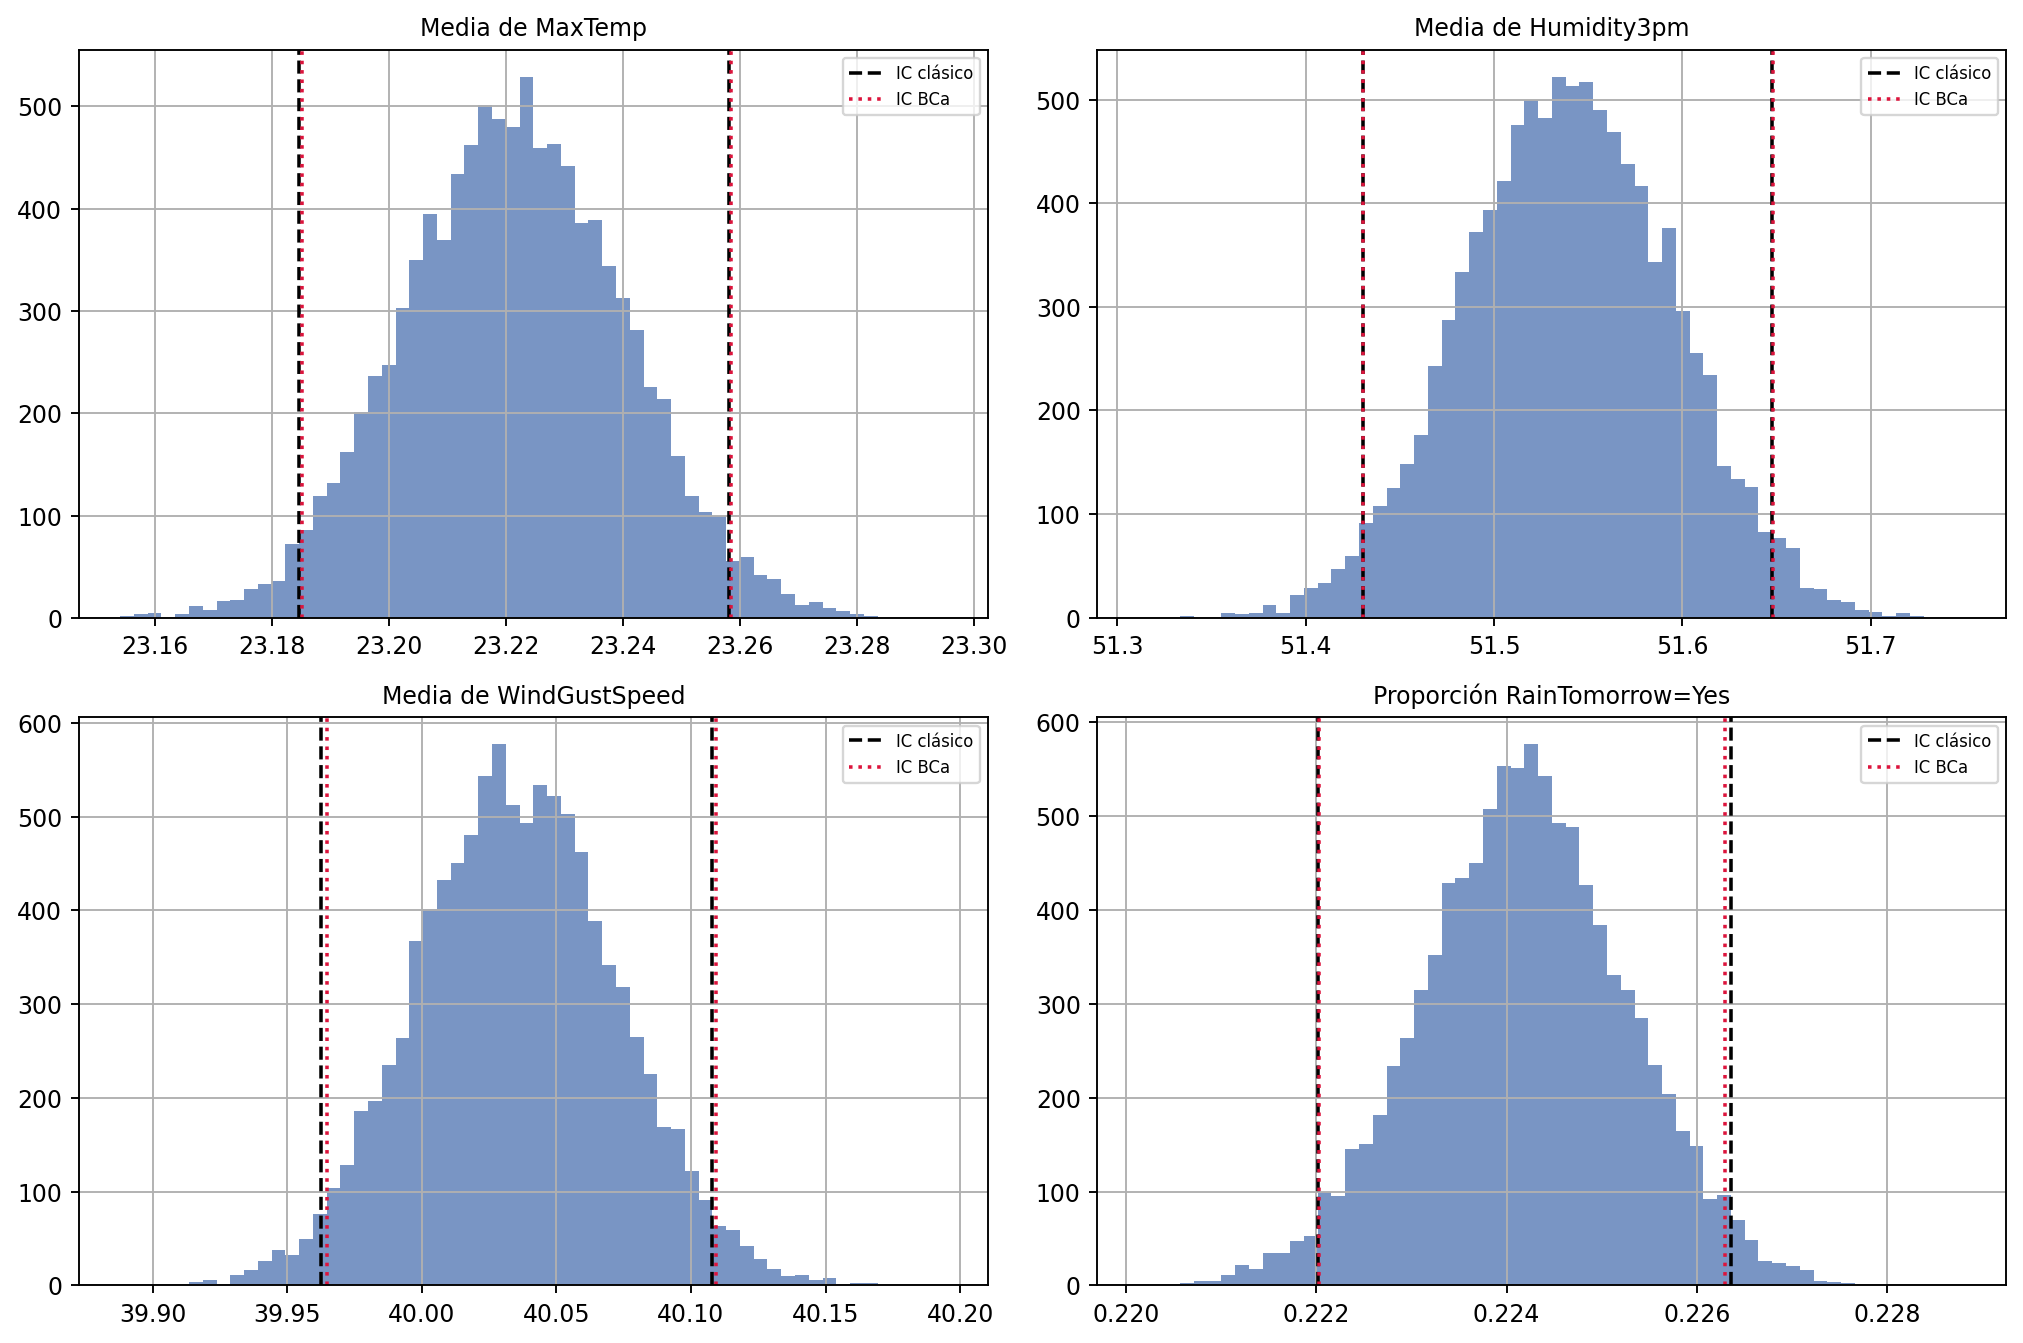
\includegraphics[width=0.87\textwidth]{../results/figures_s2/fig_s2_01_bootstrap_medias.png}
\caption{Distribuciones bootstrap e intervalos al 95\%.}
\end{figure}

\section{Validación de pruebas de hipótesis mediante permutación}

Se validaron las pruebas Welch de S1 para \texttt{MaxTemp} y \texttt{Humidity3pm} según \texttt{RainTomorrow}. En la versión corregida se utiliza un estadístico studentizado tipo Welch, no solo la diferencia directa de medias. Esto es metodológicamente consistente con S1 y adecuado ante grupos desbalanceados y varianzas potencialmente distintas.

\begin{table}[H]
\centering\footnotesize
\begin{adjustbox}{max width=\textwidth}
\begin{tabular}{lrrrrrr}
\toprule
Variable & Media Yes & Media No & Diferencia Yes-No & $t$ Welch S1 & $p$ paramétrico & $p$ permutación \\
\midrule
MaxTemp & 21.1191 & 23.8362 & -2.7171 & -61.4679 & $<0.001$ & $0.0001$ \\
Humidity3pm & 68.8000 & 46.5106 & 22.2894 & 182.6077 & $<0.001$ & $0.0001$ \\
\bottomrule
\end{tabular}
\end{adjustbox}
\caption{Comparación entre Welch de S1 y permutación studentizada de S2.}
\end{table}

El valor $p=0.0001$ corresponde al límite de resolución práctica con $10.000$ permutaciones y corrección de una unidad; por tanto se interpreta como $p<0.001$, no como cero exacto. La concordancia entre ambos enfoques refuerza las diferencias detectadas en S1, especialmente para \texttt{Humidity3pm}, cuya magnitud de efecto es alta.

\begin{figure}[H]
\centering
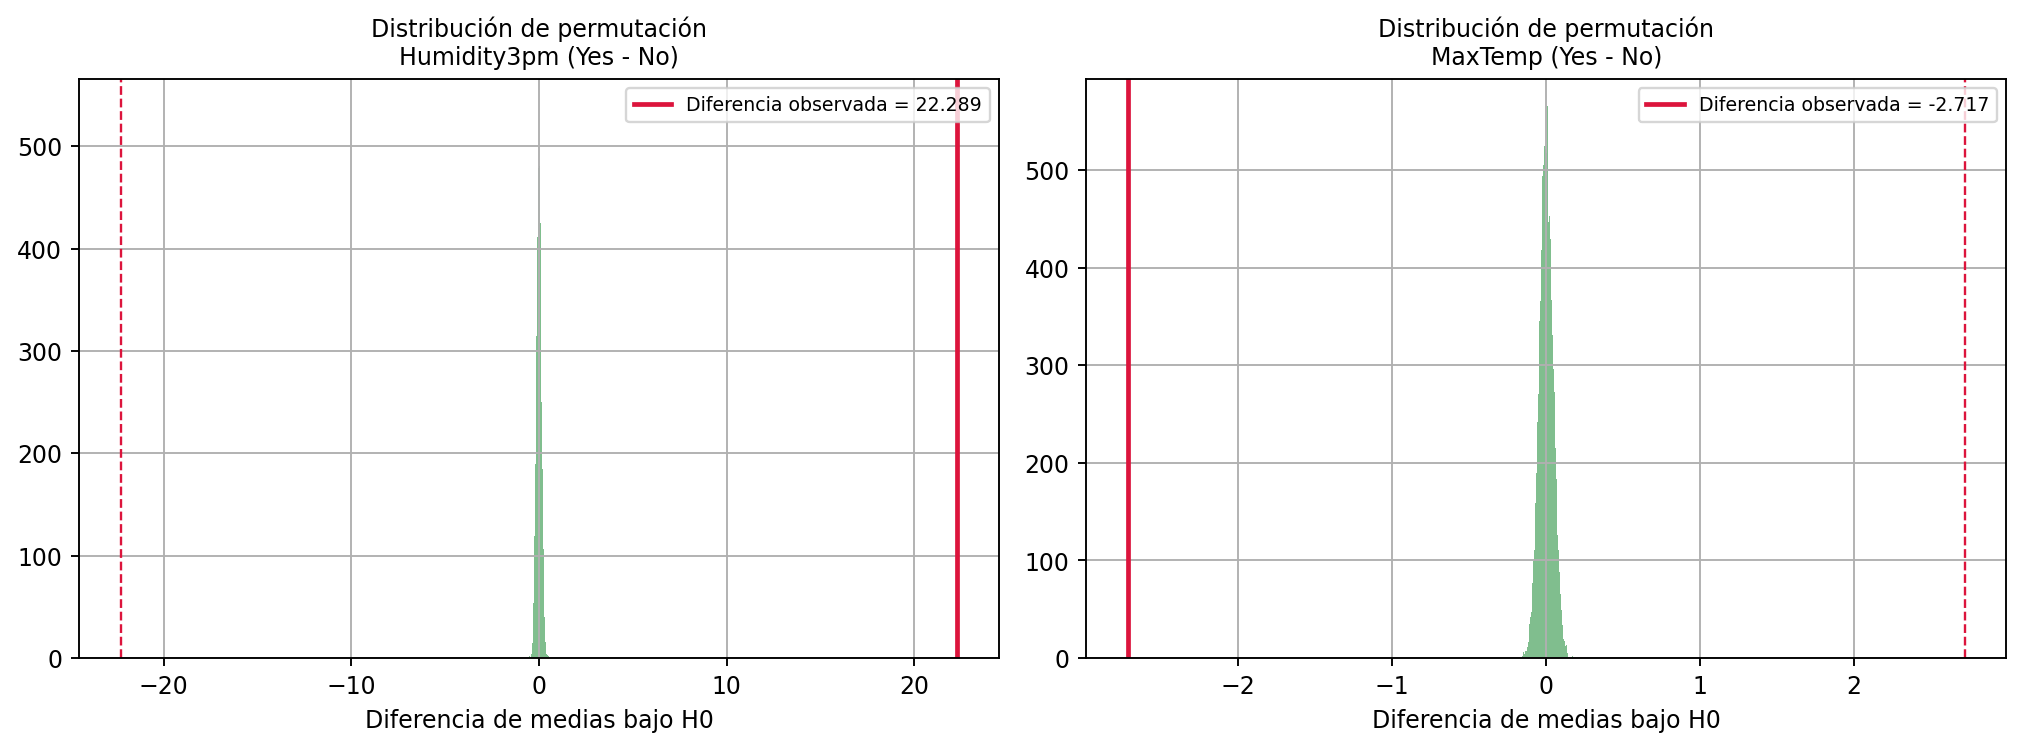
\includegraphics[width=0.86\textwidth]{../results/figures_s2/fig_s2_02_permutacion.png}
\caption{Distribuciones nulas por permutación y estadísticos observados.}
\end{figure}

\section{Evaluación de estabilidad de correlaciones}

Se seleccionaron las cinco correlaciones más relevantes de S1 con \texttt{RainTomorrow\_bin}. El bootstrap fue pareado, preservando la correspondencia entre predictor y variable objetivo.

\begin{table}[H]
\centering\footnotesize
\begin{adjustbox}{max width=\textwidth}
\begin{tabular}{lrrrrr}
\toprule
Variable & $n$ & $r$ observado & IC95 inf. & IC95 sup. & Incluye cero \\
\midrule
Humidity3pm & 138583 & 0.4462 & 0.4418 & 0.4505 & No \\
RainToday\_bin & 140787 & 0.3131 & 0.3074 & 0.3189 & No \\
Humidity9am & 140419 & 0.2572 & 0.2526 & 0.2616 & No \\
Pressure9am & 128179 & -0.2464 & -0.2516 & -0.2411 & No \\
Rainfall & 140787 & 0.2390 & 0.2319 & 0.2462 & No \\
\bottomrule
\end{tabular}
\end{adjustbox}
\caption{Estabilidad bootstrap de correlaciones relevantes de S1.}
\end{table}

Todas las correlaciones excluyen cero y se consideran estables bajo remuestreo. Además, se registra la casi colinealidad \texttt{MaxTemp}-\texttt{Temp3pm} ($r\approx0.985$), por lo que S3 no debería usar ambas variables simultáneamente sin control de colinealidad, VIF, regularización o selección previa.

\begin{figure}[H]
\centering
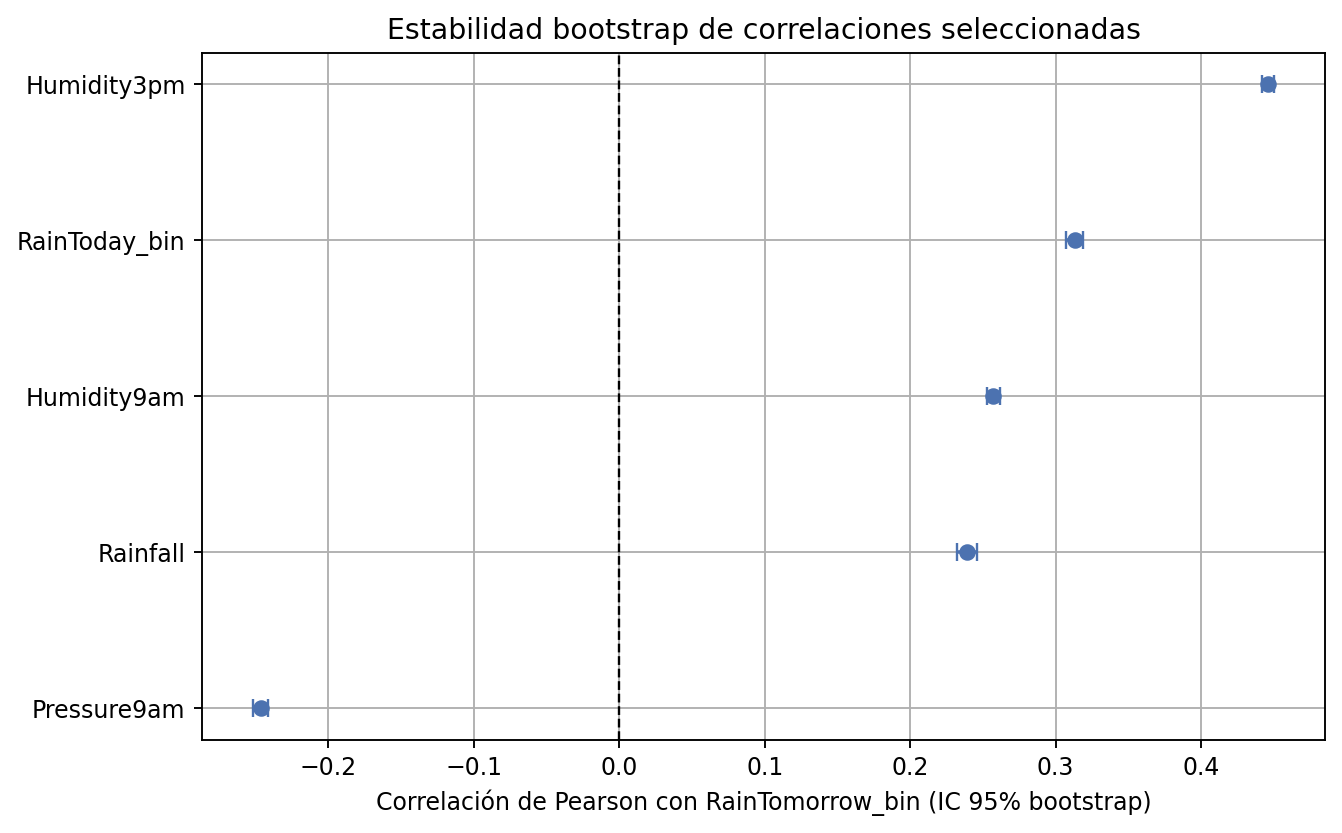
\includegraphics[width=0.76\textwidth]{../results/figures_s2/fig_s2_03_correlaciones_bootstrap.png}
\caption{Intervalos bootstrap de correlaciones con \texttt{RainTomorrow}.}
\end{figure}

\clearpage
\section{Simulación Monte Carlo basada en parámetros de S1}

Se simuló la cantidad de eventos \texttt{RainTomorrow=Yes} en 30 observaciones independientes. La probabilidad de lluvia no se fijó arbitrariamente: en cada iteración se muestreó desde la distribución bootstrap de la proporción estimada en S1 ($\hat p\approx0.2242$) y luego se aplicó un modelo binomial. Así se propaga la incertidumbre del parámetro y se responde al desbalance de clase señalado por el profesor.

\begin{table}[H]
\centering\footnotesize
\begin{tabular}{lr}
\toprule
Estadístico Monte Carlo & Resultado \\
\midrule
Número de simulaciones & 12000 \\
Ventana de observaciones & 30 \\
Media de eventos con lluvia & 6.7227 \\
Desviación estándar & 2.2826 \\
Percentil 2.5\% & 3.0000 \\
Percentil 97.5\% & 11.0000 \\
$P(Y\geq 10)$ & 0.1153 \\
$P(Y\geq 15)$ & 0.0005 \\
MCSE de la media & 0.0208 \\
\bottomrule
\end{tabular}
\caption{Resultados de la simulación Monte Carlo basada en la proporción de S1.}
\end{table}

La media simulada es coherente con $30\times0.2242\approx6.73$. Este escenario no representa un pronóstico mensual real por ciudad, pues ignora estacionalidad, localidad y dependencia temporal; se interpreta como escenario de referencia para 30 observaciones independientes bajo la frecuencia global de S1. En S3, el desbalance exige métricas como recall, precision, F1, ROC-AUC y PR-AUC, además de técnicas de remuestreo o ponderación de clases.

\begin{figure}[H]
\centering
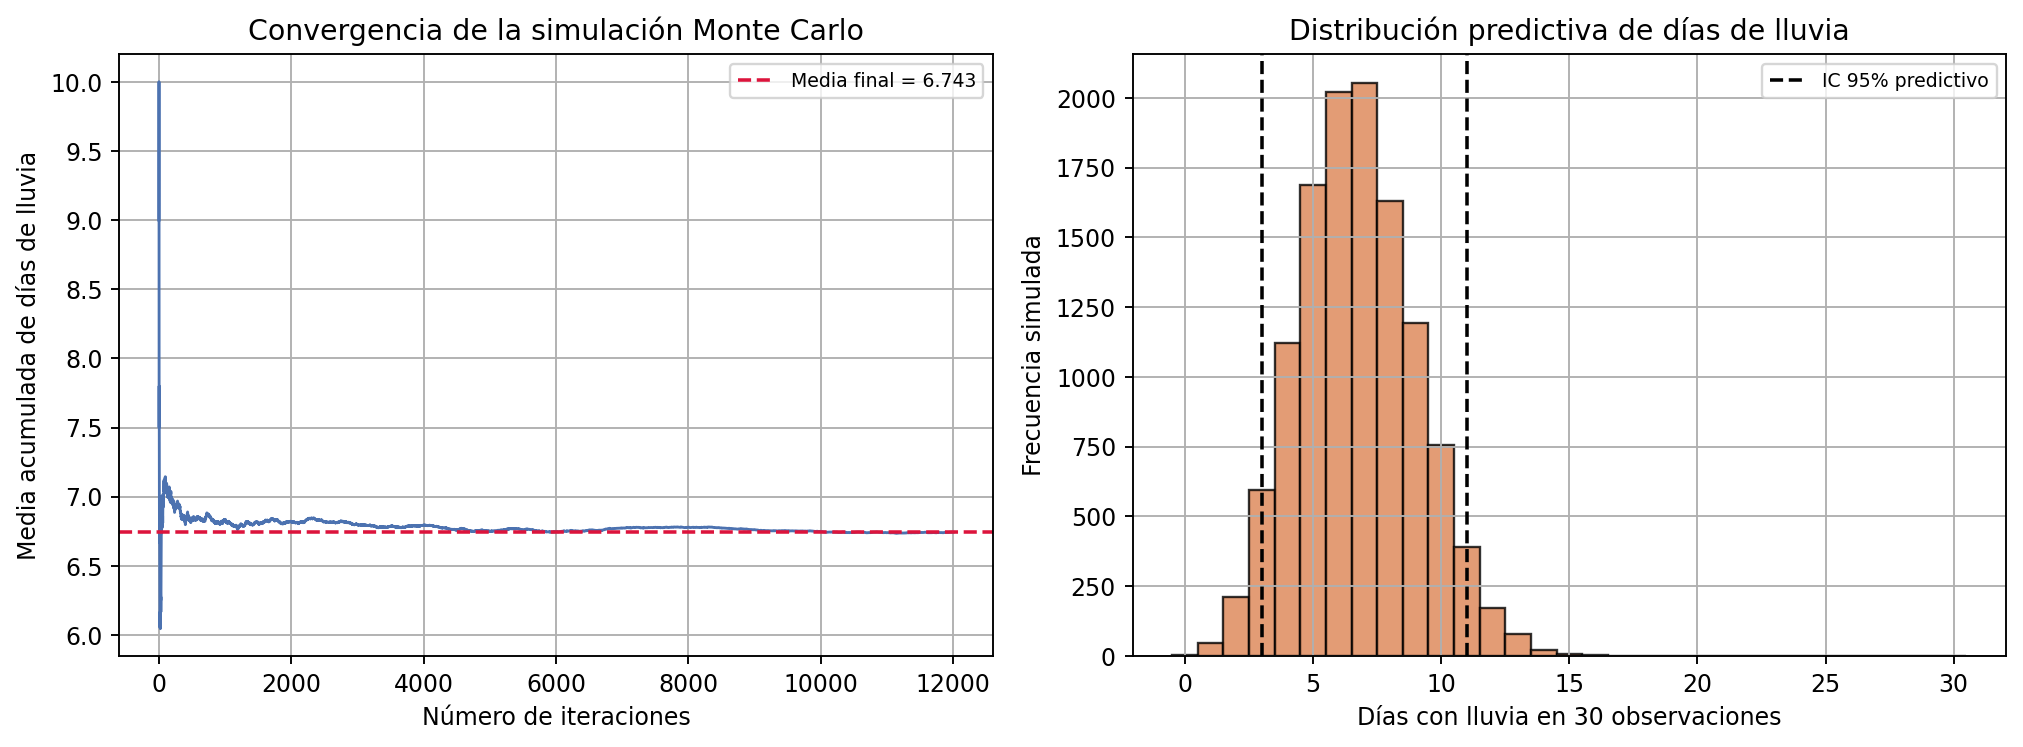
\includegraphics[width=0.86\textwidth]{../results/figures_s2/fig_s2_04_montecarlo.png}
\caption{Distribución Monte Carlo y convergencia de la media acumulada.}
\end{figure}

\section{Análisis de robustez}

La robustez se concentró en \texttt{WindGustSpeed} y \texttt{Rainfall}, tal como sugirió el profesor. Se compararon media original, media sin valores marcados por IQR, winsorización 1--99, media recortada, mediana, asimetría, curtosis y jackknife por grupos. Además, para \texttt{Rainfall} se usa \texttt{log1p}, porque la variable tiene muchos ceros y cola derecha extrema.

\begin{table}[H]
\centering\scriptsize
\begin{adjustbox}{max width=\textwidth}
\begin{tabular}{lrrrrrrr}
\toprule
Variable & $n$ & \% marcados IQR & Media original & Media sin IQR & Winsorizada & Mediana & Lectura técnica \\
\midrule
WindGustSpeed & 135197 & 2.287 & 40.035 & 39.050 & aprox. 39--40 & 39.0 & Sensibilidad moderada \\
Rainfall & 142199 & 17.987 & 2.361 & 0.155 & menor que original & 0.0 & Cero-inflada; usar cautela \\
\bottomrule
\end{tabular}
\end{adjustbox}
\caption{Robustez de variables con colas pesadas.}
\end{table}

En \texttt{WindGustSpeed}, los extremos aumentan moderadamente la media, pero los errores estándar clásico, bootstrap y jackknife son similares. En \texttt{Rainfall}, la regla IQR puede marcar gran parte de la lluvia positiva como ``outlier'' debido a la concentración de ceros; por eso no se interpreta como error de dato, sino como evidencia de asimetría estructural. Para S3 se recomienda \texttt{log1p(Rainfall)}, percentiles altos o un modelo en dos partes: ocurrencia e intensidad de lluvia.

\begin{figure}[H]
\centering
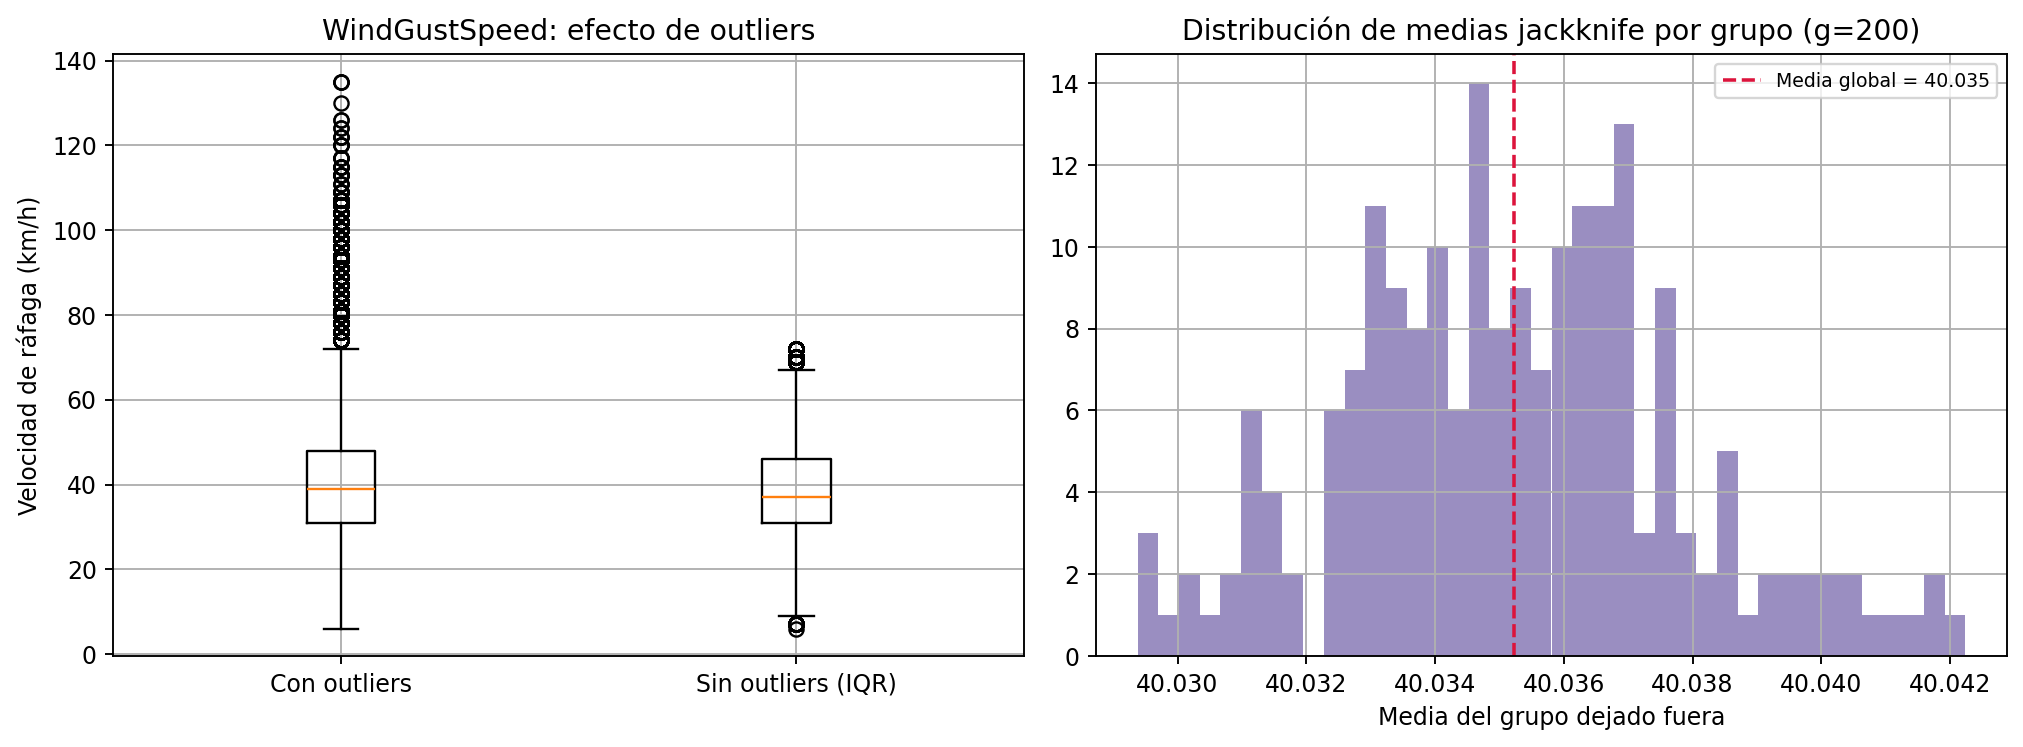
\includegraphics[width=0.86\textwidth]{../results/figures_s2/fig_s2_05_robustez.png}
\caption{Diagnóstico de robustez y jackknife.}
\end{figure}

\section{Preparación para la Sumativa 3}

\begin{itemize}
    \item \textbf{Colinealidad:} no usar \texttt{MaxTemp} y \texttt{Temp3pm} juntas sin selección, VIF o regularización.
    \item \textbf{Faltantes:} \texttt{Sunshine} y \texttt{Evaporation} requieren imputación explícita; no conviene eliminarlas por casos completos si se incorporan al modelo.
    \item \textbf{Desbalance:} \texttt{RainTomorrow=Yes} es minoritaria ($\approx22.4\%$); S3 debe usar métricas sensibles a clase minoritaria y remuestreo o ponderación.
    \item \textbf{Parámetros robustos:} \texttt{MaxTemp}, \texttt{Humidity3pm} y proporción de lluvia fueron consistentes entre IC clásico y bootstrap.
    \item \textbf{Resultados con cautela:} \texttt{Rainfall} y \texttt{WindGustSpeed} requieren métodos robustos por colas pesadas.
    \item \textbf{Dependencia:} las observaciones por estación no son independientes; S3 debería usar partición temporal o agrupada por \texttt{Location}, no solo división aleatoria simple.
\end{itemize}

El notebook corregido exporta archivos en \texttt{results/}: parámetros validados, correlaciones, pruebas de permutación, robustez de outliers, diagnóstico de colas pesadas, jackknife por \texttt{Location} y un JSON consolidado para S3.

\clearpage
\section{Bibliografía (APA 7)}
\begin{thebibliography}{9}
\bibitem{efron1993} Efron, B., \& Tibshirani, R. J. (1993). \textit{An introduction to the bootstrap}. Chapman \& Hall/CRC.
\bibitem{diciccio1996} DiCiccio, T. J., \& Efron, B. (1996). Bootstrap confidence intervals. \textit{Statistical Science, 11}(3), 189--228.
\bibitem{good2005} Good, P. I. (2005). \textit{Permutation, parametric, and bootstrap tests of hypotheses} (3rd ed.). Springer.
\bibitem{kaggle2017} Kaggle. (2017). \textit{Rain in Australia dataset}. \url{https://www.kaggle.com/datasets/jsphyg/weather-dataset-rattle-package}
\bibitem{maidana2026} Maidana, J. P. (2026). \textit{Simulación Monte Carlo, bootstrap y análisis de sensibilidad} [Apuntes de curso]. Universidad Andrés Bello.
\bibitem{virtanen2020} Virtanen, P., Gommers, R., Oliphant, T. E., et al. (2020). SciPy 1.0: Fundamental algorithms for scientific computing in Python. \textit{Nature Methods, 17}, 261--272. \url{https://doi.org/10.1038/s41592-019-0686-2}
\end{thebibliography}
\end{document}
